\documentclass{article}
\usepackage{amsmath}
\usepackage{graphicx} 
%\numberwithin{equation}{section}
\usepackage{geometry}
%\usepackage[options]{natbib}
\geometry{left=1cm,right=1cm,top=1cm,bottom=1cm}
\title{Secure Catering Paymeny Service}
\author{Shen Kai 10157891}
\begin{document}
    \maketitle
    \section{Essential components}
To simplify, we extract serveral main operations and requirements. 
This part introduce the essential parts of the whole procedures.
        \subsection*{Detailed assumptions about termials, server and cards}
%For \textbf{cards}, we assmue that each card stores one unique number which we call it \textbf{card number}. 
The card has space to store \textbf{payment secret} and the corresponding \textbf{account number}. 
Each card carries  circuits which is able to take input and generate output after some specific computation inlcuding (3DES and hash) when attached to the terminal.
For \textbf{terminals}, we assmue that each terminal store one \textbf{terminal number} and one \textbf{terminal secret number}(permanent) which is only know to the server, let's call it \textbf{TK}. 
The server stores the stuff's \textbf{account numbers} and \textbf{the hash values of their passwords} and the \textbf{payment secret}.
Termianls can also do other complex operations.
        \newline
        \subsection*{Protocol Structure}
First, there is a basic protocol to guarantee secure data transmission with shared key. 
We call it SKBSTL(shared-key-based secure tranmission layer) protocal. 
It contain three function: 
1.mutual authentication and session key generation. 
2. session key validation check. 
3.secure data transmission. (The mode decide the function in the diagram.)
Secondly other opeartion based on this protocol. 
        \newline
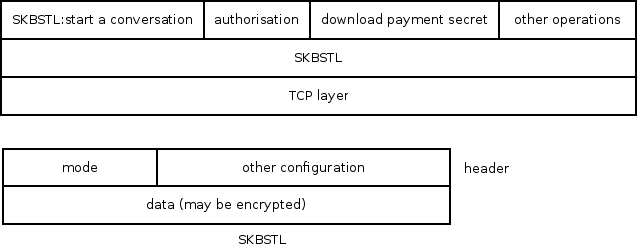
\includegraphics[width=6in]{Diagram1.png}
        \newline
        \subsection*{Mutual authentication between the Catering server and the terminal and the session key generation}
This operation happens the first time when one terminal try to communicate with the server in a period of time. 
        After the terminal and the server are both authenticated,a \textbf{session key} which is vaild for a period of time will be generated to encrypt the communication between the server and the terminal.
         The session key is stored in the terminal with a specific lifetime.
This terminal's key is also recorded in the server corresponding to its terminal number. 
        \newline
\textbf{Step 1}. First the termianl send a Mutual authentication and session key accquire request which includes its \textbf{terminal number}.
        \newline
\textbf{Step 2}. The server get the request and check if it is a legal terminal number.
Then the server send back a challenge request which includes a nouce named nouceA.
        \newline
\textbf{Step 3}. The terminal get the nouce and send back a response package which includes \textbf{  terminal number $\parallel E_{TK}[nouceA \parallel nouceB]$}. 
        \newline
\textbf{Step 4}. The server decrypt the encrypted text according to the terminal secret number stored with the termianl number and check the nouceA. 
After that, the server send back a packcage which includes  $E_{TK}[nouceB \parallel  session key(SK) \parallel E_{SK}[terminal number \parallel session key lifetime )$. 
The server stores the session key and its lifetime corresponding to the terminal number and delete the previous session key if there is one.  
        \newline
\textbf{Step 5}. The terminal encrypts the text and get the session key and its lifetime. 
After the previous communication.
The terminal and the server authenticate each other.
        \newline
\textbf{Vulnerabilities}: The attacker can keep sending  step 1 request to keep acquirring new nouce. 
This can make the legitimate user unable to authenticate itself which can be a DoS attack. 
So we make the nonce keep the same value at a period of time, we say one minute.
        \newline
\textbf{Another way}:
In step one, terminal sends the request which includes terminal numbers and $E_{TK}[current date and time \parallel nounceB]$. 
Then go straight to step 4.
    
        \subsection*{establish a confidential channel between server and terminals}
The termianl first check if it has a valid session key. 
If it does not have a valid session key. 
The terminal will do the operation \textbf{the mutual authentication between the Catering server and the terminal and the session key generation} and get the session key.
If there is a valid key. First we need to do a \textbf{the validation check}. 
\textbf{the validation check} is contained in the first two steps in the following part \textbf{start a conversation}.
If the validation check is passed, then we use the session key to guarantee the security of communication. 
        \newline
\textbf{Start a conversation} :
Then the terminal starts a conversation with the server. 
This is designed to avoid replay attack.
%the server and terminal maintain a \textbf{conversation number} according to the terminal number and the date and time. 
The server and terminal also maintains a \textbf{counter} which increases everytime there is a repuest or response between the server and the terminal.
To start a conversation.
        \newline
\textbf{Step 1}. the terminal sends a conversation establishment request which includes terminal number (which is in the SKBSTL header) and $E_{SK}[termnial number \parallel nonce0 \parallel counter = 0]$
        \newline 
\textbf{Step 2}. If the server decrypts the data and get a terminal number that is the same with the terminal number in the header, it means the validation check is passed. The server sends back a package including $terminal number and E_{SK}[nonce0 \parallel nonce1 \parallel counter = 1]$.  
        \newline
If the server decrypts the data and get a terminal number that is not the same with the terminal number in the header, then the server send a \textbf{failure information} to the terminal(which can be contained in the header). 
If the terminal only gets several failure packages after serveral tries, 
it means the current session key can not pass the validation check. 
The terminal may need to do the mutual authentication and get a new session key. 
The decision if to get a new session key is on the the terminal, 
the server will abort a valid session key only when the terminal successfully get a new one (to avoid replay attack).
(To avoid replay attack, nonceB will keep the same for a period of time.)
        \newline
\textbf{Step 3}. the terminal sends back a package including $terminal number and E_{SK}[random number \parallel nonce1 \parallel counter = 2 \parallel Data]$. 
(random numbers make it harder to decipher the ciphertext.)
        \newline
\textbf{Step 4}. Once the server gets the package, conversation is established. 
Nonce1 will be recorded and stay the same during the conversation.
The counter should be increasing. 
To tackle replay attack. Any package with the same nonce1 but less counter will be ignored.
The server aborts previous unfinished conversation with this terminal if any.
        \newline
To terminate a conversation, the terminal or server needs to exchange termiate-request package. 
Or finish the conversation automatically when timeout.
        \newline
\textbf{Integrity}:
To guarantee integrity, we can hash the data before encrypt it. TCP layer has ckecksum to tackle simple tamperring opearation.
        \newline
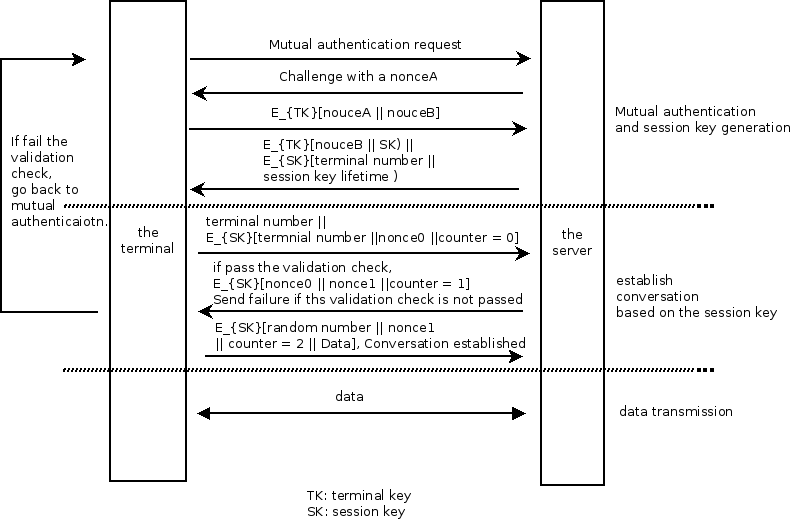
\includegraphics[width=7in]{Diagram2.png}
        \newline
        \subsection*{Secure authorisation}
This includes the operation that cards need to do,
when the card needs to send authorisation to the server. 
        \newline
First, the termianl send a request to the server. 
Then the server return a nouce(random number). 
The terminal gives this nouce to the card. 
The card uses 3DES to encrypt the nouce with the payment secret and hash it, then return to the terminal with the card number. 
The terminal send the hash value and the card number to the server. 
The server does 3DES and hash to the payment secret corresponding to the card number and compare to the value that the terminal gives if the card number is legal. 
If the check is positive. 
Then it is a legal authorisation.
    \section{Procedure: Download payment secret}
To communicate with server, the terminal needs a vaild session key. 
If there is no vaild session key recorded in the terminal or in the server for this termianl. 
Then the operation \textbf{Mutual authentication between the Catering server and the terminal and the session key generation} needs to be done first. 
If there is a vaild key and pass \textbf{the validation check},
It is possible to do next operations.
        \newline 
Alice attaches her card to the terminal. 
Terminal check if it is a leagl card (physical check). 
Ask Alice to input her account number and password. 
Alice types into her account and password. 
The terminal establishes a \textbf{conversation} with the server using its session key.
The terminal will \textbf{hash} the password and send the hash value and the account number through \textbf{the confidential channel} between server and the terminal. 
The server gets the account and checks if it is legitimate and. 
If the account is legitimate then the server compares the \textbf{hash value} with the one stored in the server. 
If the check is not passed, the server returns a failure.
If the check is passed, the server sends the \textbf{payment secret} and the \textbf{account number} of Alice through the confidential channel and payment secret will be downloaded to the card.
        \newline 
\textbf{Analysis:}
        \newline
In this procedure, the plaintext of payment secret is exposed to the terminal. 
But I think is allright because that the server sends the payment secret to the terminal only if the termianl is a legitimate one which is guaranteed by the mutul authentication and session key mechanism.
The account number and the password that Alice provides can make sure that Alice is the legitimate owner of the payment secret.
        \newline
The confidentiality of the payment secret transmission is guaranteed by the \textbf{confidential channel}. 
Though the terminal will see the plaintext of the payment secret,
we still think that it is a reliable system as we explained before.
        \newline
For \textbf{DoS}, the security is ensured by the confidential channel. 
First the attacker needs to establish a conversation with the server. 
It can not be down without a master key or a session key. 
So attackers can only do the replay attack. 
So it can never triggle the server's large-time-cost operation like searching for data in the data base,
but may triggle decrypting operation.
        \newline

    \section{Procedure: Authorised purchase}
First, the terminal establishes a conversation as before.
All the following communication is through the \textbf{confidential channel}.
Then, the terminal sends a request for authorisation.
Then, the server sends back a nonce. 
\textbf{Secure authorisation} provides the method to give authorisation. 
The card send the value $hash(E_{payment secret}[nonce])$(here we use 3DES) and Alice's account number.
The the server gets the account number and find the corresponding payment secret. 
Then the server does the opeartion $hash(E_{payment secret}[nonce])$ as well and compare the two hash values.
If then check is passed, the server send success information to the termianl. Otherwise, it sends the failure information. 
Other following information is all transferred through the \textbf{confidential channel}.
        \newline
\textbf{Analysis:}
In this procedure, the terminal can not get the payment secrect for the card hash and encrypt it. As a result, any machine tries to read the payment secret can not get that,
they can only get the hash value.
The purchase authorisation can never be re-used for the value that needs to be sent to the server is based on the nonce that the server sends.
    \section{Reference}
%@book{book1,
%    author    = "William Stallings",
%    title     = "Cryptography and Network Security: Principles and Practice 6th",
%    year      = "2013",
%    publisher = "Prentice Hall Press Upper Saddle River, NJ, USA",
%    %address   = ""
%}
[1]  William Stallings,"Cryptography and Network Security: Principles and Practice 6th",Prentice Hall Press Upper Saddle River, NJ, USA.
\end{document}
